\begin{center}
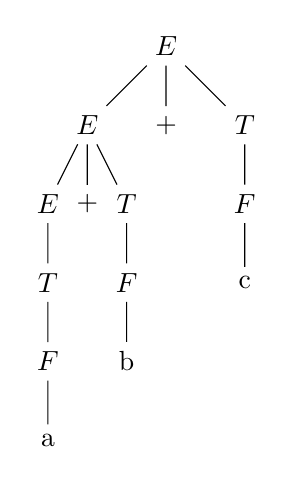
\begin{tikzpicture}[
    level distance=1cm,
    level 1/.style={sibling distance=1cm},
    level 2/.style={sibling distance=0.5cm}
]
    \node {$E$}
    child {node {$E$}
        child {node {$E$}
            child {node {$T$}
                child {node {$F$}
                    child {node {\str{a}}
                    }
                }
            }
        }
        child {node {\str{+}}}
        child {node {$T$}
            child {node {$F$}
                child {node {\str{b}}
                }
            }
        }
    }
    child {node {\str{+}}}
    child {node {$T$}
        child {node {$F$}
            child {node {\str{c}}}
        }
    };
\end{tikzpicture}
\end{center}